%!TEX TS-program = xelatex
\documentclass[12pt, a4paper, oneside]{article}

\usepackage{amsmath,amsfonts,amssymb,amsthm,mathtools}  % пакеты для математики

\usepackage[english, russian]{babel} % выбор языка для документа
\usepackage[utf8]{inputenc} % задание utf8 кодировки исходного tex файла
\usepackage[X2,T2A]{fontenc}        % кодировка

\usepackage{fontspec}         % пакет для подгрузки шрифтов
\setmainfont{Linux Libertine O}   % задаёт основной шрифт документа

\usepackage{unicode-math}     % пакет для установки математического шрифта
\setmathfont[math-style=upright]{Neo Euler} % шрифт для математики

% Конкретный символ из конкретного шрифта
% \setmathfont[range=\int]{Neo Euler}

%%%%%%%%%% Работа с картинками %%%%%%%%%
\usepackage{graphicx}                  % Для вставки рисунков
\usepackage{graphics}
\graphicspath{{images/}{pictures/}}    % можно указать папки с картинками
\usepackage{wrapfig}                   % Обтекание рисунков и таблиц текстом

%%%%%%%%%%%%%%%%%%%%%%%% Графики и рисование %%%%%%%%%%%%%%%%%%%%%%%%%%%%%%%%%
\usepackage{tikz, pgfplots}  % язык для рисования графики из latex'a

%%%%%%%%%% Гиперссылки %%%%%%%%%%
\usepackage{xcolor}              % разные цвета

\usepackage{hyperref}
\hypersetup{
	unicode=true,           % позволяет использовать юникодные символы
	colorlinks=true,       	% true - цветные ссылки, false - ссылки в рамках
	urlcolor=blue,          % цвет ссылки на url
	linkcolor=red,          % внутренние ссылки
	citecolor=green,        % на библиографию
	pdfnewwindow=true,      % при щелчке в pdf на ссылку откроется новый pdf
	breaklinks              % если ссылка не умещается в одну строку, разбивать ли ее на две части?
}


\usepackage{todonotes} % для вставки в документ заметок о том, что осталось сделать
% \todo{Здесь надо коэффициенты исправить}
% \missingfigure{Здесь будет Последний день Помпеи}
% \listoftodos --- печатает все поставленные \todo'шки

\usepackage[paper=a4paper, top=20mm, bottom=15mm,left=20mm,right=15mm]{geometry}
\usepackage{indentfirst}       % установка отступа в первом абзаце главы

\usepackage{setspace}
\setstretch{1.15}  % Межстрочный интервал
\setlength{\parskip}{4mm}   % Расстояние между абзацами
% Разные длины в латехе https://en.wikibooks.org/wiki/LaTeX/Lengths


\usepackage{xcolor} % Enabling mixing colors and color's call by 'svgnames'

\definecolor{MyColor1}{rgb}{0.2,0.4,0.6} %mix personal color
\newcommand{\textb}{\color{Black} \usefont{OT1}{lmss}{m}{n}}
\newcommand{\blue}{\color{MyColor1} \usefont{OT1}{lmss}{m}{n}}
\newcommand{\blueb}{\color{MyColor1} \usefont{OT1}{lmss}{b}{n}}
\newcommand{\red}{\color{LightCoral} \usefont{OT1}{lmss}{m}{n}}
\newcommand{\green}{\color{Turquoise} \usefont{OT1}{lmss}{m}{n}}

\usepackage{titlesec}
\usepackage{sectsty}
%%%%%%%%%%%%%%%%%%%%%%%%
%set section/subsections HEADINGS font and color
\sectionfont{\color{MyColor1}}  % sets colour of sections
\subsectionfont{\color{MyColor1}}  % sets colour of sections

%set section enumerator to arabic number (see footnotes markings alternatives)
\renewcommand\thesection{\arabic{section}.} %define sections numbering
\renewcommand\thesubsection{\thesection\arabic{subsection}} %subsec.num.

%define new section style
\newcommand{\mysection}{
	\titleformat{\section} [runin] {\usefont{OT1}{lmss}{b}{n}\color{MyColor1}} 
	{\thesection} {3pt} {} } 


%	CAPTIONS
\usepackage{caption}
\usepackage{subcaption}
%%%%%%%%%%%%%%%%%%%%%%%%
\captionsetup[figure]{labelfont={color=Turquoise}}

\pagestyle{empty}

%%%%%%%%%% Свои команды %%%%%%%%%%
\usepackage{etoolbox}    % логические операторы для своих макросов

% Все свои команды лучше всего определять не по ходу текста, как это сделано в этом документе, а в преамбуле!

% Одно из применений - уничтожение какого-то куска текста!
\newbool{answers}
\booltrue{answers}
%\boolfalse{answers}

\usepackage{enumitem}
% бульпоинты в списках
\definecolor{myblue}{rgb}{0, 0.45, 0.70}
\newcommand*{\MyPoint}{\tikz \draw [baseline, fill=myblue,draw=blue] circle (2.5pt);}
\renewcommand{\labelitemi}{\MyPoint}

% расстояние в списках
\setlist[itemize]{parsep=0.4em,itemsep=0em,topsep=0ex}
\setlist[enumerate]{parsep=0.4em,itemsep=0em,topsep=0ex}


\begin{document}
	
\section*{Семинар 3: Немного математики}

\subsection*{Задача 1 (Ищем вероятности)}

Давайте решим несколько задачек на вероятности! 

\begin{enumerate}
\item  Драгомир принёс на пару кубик и подкинул его. Какова вероятность того, что на кубике выпадет число $6$? Какова вероятность того, что на кубике выпадет чётное число? 

\item  Витя очень классный! Маша записала в столовой его номер телефона на салфетке. К сожалению, последние две цифры затёрлись. Маша помнит, что одна из цифр в конце ноль, а вторая нечётная. Какова вероятность, что Маша наберёт правильный телефон с первого раза? 

\item  Добрыня, Илья и Алёша приехали на пару на кирпич и зашли в лифт. Лифт не сломался и едет наверх. В кирпиче $20$ этажей. Какова вероятность, что парни выйдут на одном этаже? Какова вероятность, что парни выйдут на разных этажах? Какова вероятность, что двое из них выйдут на одном этаже. \textbf{Hint:} в сумме эти три вероятности дают один. 

\item Задача, которой на самом первом собеседовании по телефону в Яндекс HR проверяют, надо ли бросить трубку.  Монетку подбросили $5$ раз. Какова вероятность, что орёл на ней выпадет все $5$ раз? Какова вероятность того, что орёл выпал $1$ раз, а решка $4$ раза?
\end{enumerate}

\subsection*{Задача 2 (Ищем математическое ожидание)}

Дима участвует в лотерее. Он знает, что на $20000$ билетов всего $1$ выигрышный. Дима участвует в игре каждую неделю. Билет стоит $100$ рублей. Выиграть можно $1000000$ рублей. Найдите ожидаемые доходы (или убытки) Димы. 


\subsection*{Задача 3 (Расстояния)}

Война за железный трон спустилась на 7 королевств. Армия Станиса Баратеона остановилась в крепости Драконий Камень. Армия Тайвина Ланистера стоит в разрушенной крепости Харренхолле. Армия Роба Старка оказалась в лесу. Единственному истинному королю и наследнику трона Станису Баратеону нужно решить по кому нанести удар. К счастью у него в свите оказалась леди Мелисандра, знакомая с математикой. 

\begin{enumerate}
\item[а)]  Красная женщина начертила огнём в воздухе систему координат и выяснила, что в ней Станис находится в точке $A(1,1)$. Ланистеры в точке $B(2,2)$. Старки в точке $C(3,0)$. Изобразите все три точки на картинке.

\item[б)]  Бог Света предлагает Станису использовать для поиска расстояния евклидову метрику. До чьей армии ближе идти, чтобы атаковать? 

\item[в)]  Старые боги предлагают Станису использовать манхеттенскую метрику для поиска расстояния. До кого ближе идти, чтобы атаковать?  Каких богов вы бы послушали и почему? 

\item[г)] Какое расстояние будете использовать для того, чтобы добраться из точки А в точку Б? Почему? 

\begin{minipage}[t]{0.45\textwidth}
	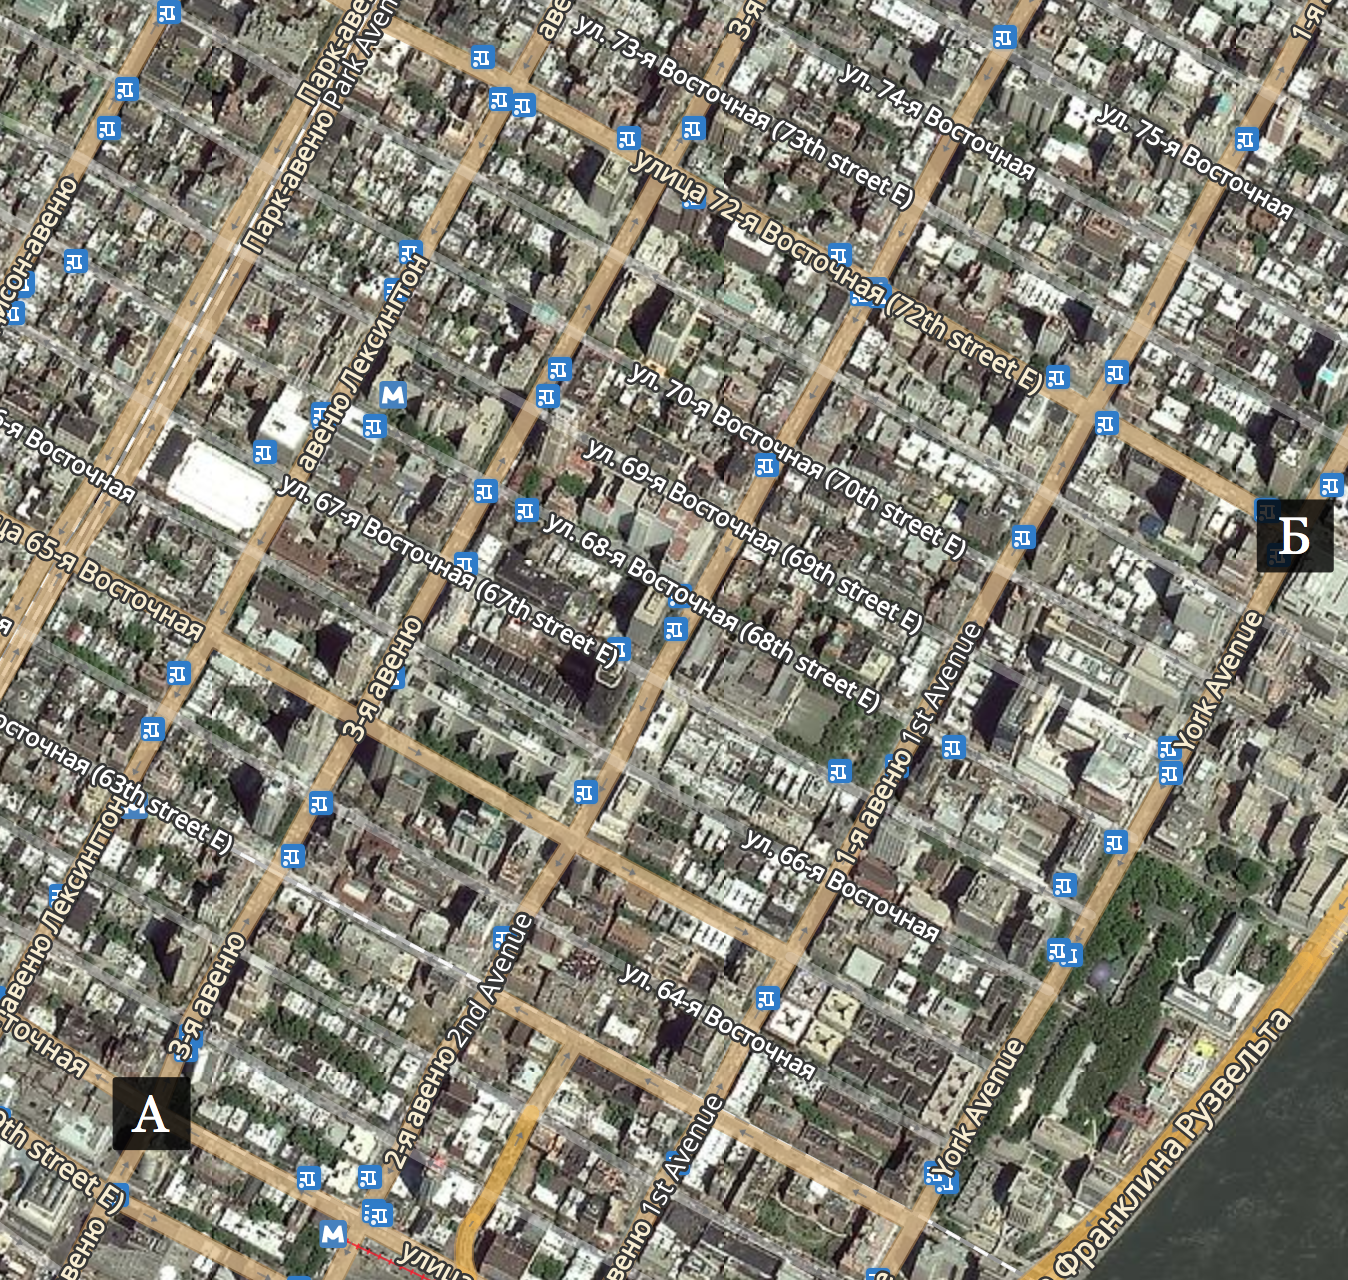
\includegraphics[scale=0.12]{metr_1.png}
\end{minipage}
\hfill
\begin{minipage}[t]{0.45\textwidth}
	\includegraphics[scale=0.13]{metr_2.png}
\end{minipage}

\end{enumerate}





\end{document}
